\begin{frame}[t,allowframebreaks,allowdisplaybreaks]
    \frametitle{B-Tree Operations---Search (Example)}
    \newcounter{search-example}
    \newcounter{search-img-example}
    \newcounter{search-step-example}[search-example]
    \setcounter{search-example}{0}
    \setcounter{search-img-example}{0}
    \setcounter{search-step-example}{0}
    % Search 1
    \stepcounter{search-example}
    \stepcounter{search-img-example}
	\stepcounter{search-step-example}
    \begin{columns}
        \begin{column}{.47\textwidth}
            \inputminted[%
                highlightlines={1,2,3,4},%
                firstline=1,%
                lastline=5,%
                tabsize=1,%
                fontsize=\examplefnt,%
            ]{c}{resources/code/b_tree_find.c}
        \end{column}
        \begin{column}{.5\textwidth}
            \examplefnt{%
                \begin{itemize}
                    \item Search \arabic{search-example}; Step \arabic{search-step-example};
                    \item tree=(*pag 0); \hlght{query\_key=70;}
                    \item object;
                    \item \hlght{current\_node=(*pag 0);}
                \end{itemize}
            }
        \end{column}
    \end{columns}
    \begin{figure}[h!]
        \includegraphics[%
            height=0.65\textheight,%
            page=\value{search-img-example}%
        ]{resources/made/B-Trees_search_example.pdf}
    \end{figure}
    \framebreak{}
    \stepcounter{search-img-example}
	\stepcounter{search-step-example}
    \begin{columns}
        \begin{column}{.47\textwidth}
            \inputminted[%
                highlightlines={6,9,10},%
                firstline=6,%
                lastline=11,%
                tabsize=1,%
                fontsize=\examplefnt,%
            ]{c}{resources/code/b_tree_find.c}
        \end{column}
        \begin{column}{.5\textwidth}
            \examplefnt{%
                \begin{itemize}
                    \item Search \arabic{search-example}; Step \arabic{search-step-example};
                    \item tree=(*pag 0); query\_key=70;
                    \item object; \hlght{lower=0; upper=2;}
                    \item current\_node=(*pag 0);
                \end{itemize}
            }
        \end{column}
    \end{columns}
    \begin{figure}[h!]
        \includegraphics[%
            height=0.65\textheight,%
            page=\value{search-img-example}%
        ]{resources/made/B-Trees_search_example.pdf}
    \end{figure}
    \framebreak{}
    \stepcounter{search-img-example}
	\stepcounter{search-step-example}
    \begin{columns}
        \begin{column}{.47\textwidth}
            \inputminted[%
                highlightlines={12,13,14,17},%
                firstline=12,%
                lastline=18,%
                tabsize=1,%
                fontsize=\examplefnt,%
            ]{c}{resources/code/b_tree_find.c}
        \end{column}
        \begin{column}{.5\textwidth}
            \examplefnt{%
                \begin{itemize}
                    \item Search \arabic{search-example}; Step \arabic{search-step-example};
                    \item tree=(*pag 0); query\_key=70;
                    \item object; \hlght{lower=0 \rarr{} 1; upper=2; med=1;}
                    \item current\_node=(*pag 0);
                \end{itemize}
            }
        \end{column}
    \end{columns}
    \begin{figure}[h!]
        \includegraphics[%
            height=0.65\textheight,%
            page=\value{search-img-example}%
        ]{resources/made/B-Trees_search_example.pdf}
    \end{figure}
    \framebreak{}
    \stepcounter{search-img-example}
	\stepcounter{search-step-example}
    \begin{columns}
        \begin{column}{.47\textwidth}
            \inputminted[%
                highlightlines={12},%
                firstline=12,%
                lastline=12,%
                tabsize=1,%
                fontsize=\examplefnt,%
            ]{c}{resources/code/b_tree_find.c}
            \inputminted[%
                highlightlines={19,20},%
                firstline=18,%
                lastline=21,%
                tabsize=1,%
                fontsize=\examplefnt,%
            ]{c}{resources/code/b_tree_find.c}
        \end{column}
        \begin{column}{.5\textwidth}
            \examplefnt{%
                \begin{itemize}
                    \item Search \arabic{search-example}; Step \arabic{search-step-example};
                    \item tree=(*pag 0); query\_key=70;
                    \item object; \hlght{lower=1; upper=2;}
                    \item \hlght{current\_node=(*pag 0) \rarr{} (*pag 5);}
                \end{itemize}
            }
        \end{column}
    \end{columns}
    \begin{figure}[h!]
        \includegraphics[%
            height=0.65\textheight,%
            page=\value{search-img-example}%
        ]{resources/made/B-Trees_search_example.pdf}
    \end{figure}
    \framebreak{}
    \stepcounter{search-img-example}
	\stepcounter{search-step-example}
    \begin{columns}
        \begin{column}{.47\textwidth}
            \inputminted[%
                highlightlines={9,10},%
                firstline=6,%
                lastline=10,%
                tabsize=1,%
                fontsize=\examplefnt,%
            ]{c}{resources/code/b_tree_find.c}
        \end{column}
        \begin{column}{.5\textwidth}
            \examplefnt{%
                \begin{itemize}
                    \item Search \arabic{search-example}; Step \arabic{search-step-example};
                    \item tree=(*pag 0); query\_key=70;
                    \item object; \hlght{lower=0; upper=2;}
                    \item current\_node=(*pag 5);
                \end{itemize}
            }
        \end{column}
    \end{columns}
    \begin{figure}[h!]
        \includegraphics[%
            height=0.65\textheight,%
            page=\value{search-img-example}%
        ]{resources/made/B-Trees_search_example.pdf}
    \end{figure}
    \framebreak{}
    \stepcounter{search-img-example}
	\stepcounter{search-step-example}
    \begin{columns}
        \begin{column}{.47\textwidth}
            \inputminted[%
                highlightlines={14,17},%
                firstline=12,%
                lastline=18,%
                tabsize=1,%
                fontsize=\examplefnt,%
            ]{c}{resources/code/b_tree_find.c}
        \end{column}
        \begin{column}{.5\textwidth}
            \examplefnt{%
                \begin{itemize}
                    \item Search \arabic{search-example}; Step \arabic{search-step-example};
                    \item tree=(*pag 0); query\_key=70;
                    \item object; \hlght{lower=0 \rarr{} 1;} upper=2; \hlght{med=1;}
                    \item current\_node=(*pag 5);
                \end{itemize}
            }
        \end{column}
    \end{columns}
    \begin{figure}[h!]
        \includegraphics[%
            height=0.65\textheight,%
            page=\value{search-img-example}%
        ]{resources/made/B-Trees_search_example.pdf}
    \end{figure}
    \framebreak{}
    \stepcounter{search-img-example}
	\stepcounter{search-step-example}
    \begin{columns}
        \begin{column}{.47\textwidth}
            \inputminted[%
                highlightlines={12},%
                firstline=12,%
                lastline=12,%
                tabsize=1,%
                fontsize=\examplefnt,%
            ]{c}{resources/code/b_tree_find.c}
            \inputminted[%
                highlightlines={20},%
                firstline=18,%
                lastline=21,%
                tabsize=1,%
                fontsize=\examplefnt,%
            ]{c}{resources/code/b_tree_find.c}
        \end{column}
        \begin{column}{.5\textwidth}
            \examplefnt{%
                \begin{itemize}
                    \item Search \arabic{search-example}; Step \arabic{search-step-example};
                    \item tree=(*pag 0); query\_key=70;
                    \item object; \hlght{lower=1;} upper=2;
                    \item \hlght{current\_node=(*pag 5) \rarr{} (*pag 4);}
                \end{itemize}
            }
        \end{column}
    \end{columns}
    \begin{figure}[h!]
        \includegraphics[%
            height=0.65\textheight,%
            page=\value{search-img-example}%
        ]{resources/made/B-Trees_search_example.pdf}
    \end{figure}
    \framebreak{}
    \stepcounter{search-img-example}
	\stepcounter{search-step-example}
    \begin{columns}
        \begin{column}{.47\textwidth}
            \inputminted[%
                highlightlines={9,10},%
                firstline=6,%
                lastline=10,%
                tabsize=1,%
                fontsize=\examplefnt,%
            ]{c}{resources/code/b_tree_find.c}
        \end{column}
        \begin{column}{.5\textwidth}
            \examplefnt{%
                \begin{itemize}
                    \item Search \arabic{search-example}; Step \arabic{search-step-example};
                    \item tree=(*pag 0); query\_key=70;
                    \item object; \hlght{lower=0; upper=2;}
                    \item current\_node=(*pag 4);
                \end{itemize}
            }
        \end{column}
    \end{columns}
    \begin{figure}[h!]
        \includegraphics[%
            height=0.65\textheight,%
            page=\value{search-img-example}%
        ]{resources/made/B-Trees_search_example.pdf}
    \end{figure}
    \framebreak{}
    \stepcounter{search-img-example}
	\stepcounter{search-step-example}
    \begin{columns}
        \begin{column}{.47\textwidth}
            \inputminted[%
                highlightlines={14,15},%
                firstline=12,%
                lastline=18,%
                tabsize=1,%
                fontsize=\examplefnt,%
            ]{c}{resources/code/b_tree_find.c}
        \end{column}
        \begin{column}{.5\textwidth}
            \examplefnt{%
                \begin{itemize}
                    \item Search \arabic{search-example}; Step \arabic{search-step-example};
                    \item tree=(*pag 0); query\_key=70;
                    \item object; \hlght{lower=0; upper=2 \rarr{} 1; med=1;}
                    \item current\_node=(*pag 4);
                \end{itemize}
            }
        \end{column}
    \end{columns}
    \begin{figure}[h!]
        \includegraphics[%
            height=0.65\textheight,%
            page=\value{search-img-example}%
        ]{resources/made/B-Trees_search_example.pdf}
    \end{figure}
    \framebreak{}
    \stepcounter{search-img-example}
	\stepcounter{search-step-example}
    \begin{columns}
        \begin{column}{.47\textwidth}
            \inputminted[%
                highlightlines={12},%
                firstline=12,%
                lastline=12,%
                tabsize=1,%
                fontsize=\examplefnt,%
            ]{c}{resources/code/b_tree_find.c}
            \inputminted[%
                highlightlines={19},%
                firstline=19,%
                lastline=19,%
                tabsize=1,%
                fontsize=\examplefnt,%
            ]{c}{resources/code/b_tree_find.c}
            \inputminted[%
                highlightlines={23,24,27},%
                firstline=22,%
                lastline=28,%
                tabsize=1,%
                fontsize=\examplefnt,%
            ]{c}{resources/code/b_tree_find.c}
        \end{column}
        \begin{column}{.5\textwidth}
            \examplefnt{%
                \begin{itemize}
                    \item Search \arabic{search-example}; Step \arabic{search-step-example};
                    \item tree=(*pag 0); query\_key=70;
                    \item \hlght{lower=0;} upper=1;
                    \item current\_node=(*pag 4);
                    \item \hlght{object=(*70);}
                \end{itemize}
            }
        \end{column}
    \end{columns}
    \begin{figure}[h!]
        \includegraphics[%
            height=0.5\textheight,%
            page=\value{search-img-example}%
        ]{resources/made/B-Trees_search_example.pdf}
    \end{figure}
\end{frame}
